\documentclass[compress]{beamer}

\usepackage[nofonts]{ctex}
\setCJKmainfont[ItalicFont={Kaiti SC}]{Kaiti SC}%
%\setCJKmainfont[ItalicFont={AR PL KaitiM GB}]{AR PL KaitiM GB}%
%\setCJKsansfont{WenQuanYi Zen Hei}% 文泉驿的黑体

\mode<beamer>
{
     \useinnertheme{rectangles}
     %\useoutertheme{infolines}
     %\useoutertheme{split}
     \usecolortheme{rose}
     \usecolortheme{seahorse}

     \setbeamertemplate{navigation symbols}{}%remove navigation symbols

     %\expandafter\def\expandafter\insertshorttitle\expandafter{%
     %\insertshorttitle\hfill%
     %\insertframenumber\,/\,\inserttotalframenumber}
     %\raisebox{-1ex}{
\includegraphics[width=3ex]{Overlays/logo.pdf}}}
     \setbeamertemplate{footline} {
      \leavevmode%
      \hbox{%
      \begin{beamercolorbox}[wd=.1\paperwidth,ht=2.25ex,dp=1ex,left]{date in head/foot}%
        \usebeamerfont{date in head/foot}%
        \hspace*{1ex}\raisebox{-0.8ex}{
\includegraphics[width=3ex]{Overlays/logo.pdf}}%
      \end{beamercolorbox}%
      \begin{beamercolorbox}[wd=.4\paperwidth,ht=2.25ex,dp=1ex,right]{date in head/foot}%
        \usebeamerfont{date in head/foot}\insertsection\hspace*{1ex}
      \end{beamercolorbox}%
      \begin{beamercolorbox}[wd=.4\paperwidth,ht=2.25ex,dp=1ex,left]{date in head/foot}%
        \usebeamerfont{date in head/foot}\hspace*{1ex}\insertsubsection
      \end{beamercolorbox}%
      \begin{beamercolorbox}[wd=.1\paperwidth,ht=2.25ex,dp=1ex,right]{date in head/foot}%
        \insertframenumber{} / \inserttotalframenumber\hspace*{1ex}
      \end{beamercolorbox}}%
      \vskip0pt%
    }

}

%\defbeamertemplate*{footline}{mytheme}
%{
%  \leavevmode%
%  \hbox{%
%  \begin{beamercolorbox}[wd=.5\paperwidth,ht=2.25ex,dp=1ex,center]{author in head/foot}%
%    \usebeamerfont{author in head/foot}\insertshortauthor~~%
%    \raisebox{-1ex}{
\includegraphics[width=3ex]{Overlays/logo.pdf}}%
%  \end{beamercolorbox}%
%  \begin{beamercolorbox}[wd=.5\paperwidth,ht=2.25ex,dp=1ex,right]{title in head/foot}%
%    \usebeamerfont{title in head/foot}\insertshorttitle{}\hspace*{2em}
%    \insertframenumber{} / \inserttotalframenumber\hspace*{2ex} 
%  \end{beamercolorbox}}%
%  \vskip0pt%
%}
%\usebeamertemplate{mytheme}

\mode<handout>
{
	\usetheme{default}
	\usepackage{pgfpages}
	\pgfpagesuselayout{4 on 1}[a4paper,landscape,border shrink=5mm]
}


\usepackage{amsmath,latexsym,amssymb,amsfonts,amsbsy}
\usepackage{graphicx}
\usepackage{hyperref}
\usepackage{textpos}
\usepackage{comment}
\usepackage{fancyvrb}
\fvset{frame=single, numbers=left, fontsize=\small}
\usepackage{tikz}
\usetikzlibrary{calc,arrows.meta, graphs, trees, shapes, positioning,
decorations.markings, intersections, decorations.text}
\usepackage{tikz-uml}


\newcommand{\romannumber}[1]{{\textrm{\uppercase\expandafter{\romannumeral
#1}}}}

\graphicspath{{figure/}}

%%%%%%%%%%%%%%%%%%%%%%%%%%%%%%%%%%%%%%%%%%%%%%%%%%%%%%%%%%%%%%%%%
%    body                                                       %
%%%%%%%%%%%%%%%%%%%%%%%%%%%%%%%%%%%%%%%%%%%%%%%%%%%%%%%%%%%%%%%%%


\begin{document}

\AtBeginSection[]
{ 
    \begin{frame}<beamer> 
		\frametitle{内容提要} 
		\tableofcontents[currentsection,currentsubsection,
        subsectionstyle=show/shaded/hide] 
	\end{frame} 
} 

					
\title{第一章 ~~ 面向对象方法概论}

\author[面向对象的分析与设计]
{曹东刚\\\href{mailto:caodg@pku.edu.cn}{caodg@pku.edu.cn}}

\institute[北京大学]{北京大学信息学院研究生课程 - 面向对象的分析与设计}


\date{}

\titlegraphic{
\includegraphics[height=0.1\textwidth]{Overlays/logo.pdf}}

\begin{frame}[plain]
	\titlepage
\end{frame}

%\includeonlyframes{current}

\setcounter{framenumber}{0}

\section{认识对象}

\subsection{定义}

\begin{frame}
\frametitle{什么是面向对象}
\begin{block}{从程序设计的角度}
面向对象是一种新的程序设计范型(paradigm),其基本思想是使用对象、类、继承
、封装、聚合、关联、消息、多态性等基本概念来进行程序设计
\end{block}
\end{frame}

\begin{frame}
    \frametitle{关于编程范型}

\begin{block}{编程范型 -- From Wikipedia}
    A programming paradigm is a fundamental style of computer
    programming, serving as a way of building the structure and elements
    of computer programs. 
\end{block}

    Programming paradigms that are often distinguished include
    \textbf{imperative, declarative, functional, object-oriented}, procedural,
    logic and symbolic programming.


\end{frame}

\begin{frame}
\frametitle{什么是面向对象}

\begin{block}{从软件开发的角度}
面向对象不仅是一些具体的软件开发技术与策略,而且是一整套关于如何看待软件系统与
现实世界的关系,用什么观点来研究问题并进行问题求解,以及如何进行系统构造
的软件方法学
\end{block}

\pause

\begin{block}{定义}
面向对象是一种运用对象、类、继承、封装、聚合、关联、消息、多态性等概
念来构造系统的软件开发方法
\end{block}
\end{frame}

%\begin{frame}
    %\frametitle{什么是软件方法学}
    %\begin{block}{Software Development Methodology-- From Wikipedia}
       %In software engineering, a software development methodology 
       %is a division of software development work into distinct phases (or
       %stages) containing activities with the intent of better planning
       %and management. 
    %\end{block}
%
       %Common methodologies include waterfall, prototyping, iterative
       %and incremental development, spiral development, rapid
       %application development, extreme programming and agile
       %methodology.
%\end{frame}


\begin{frame}
  \frametitle{软件开发核心的问题是复杂性控制}
  \begin{center}
    \centering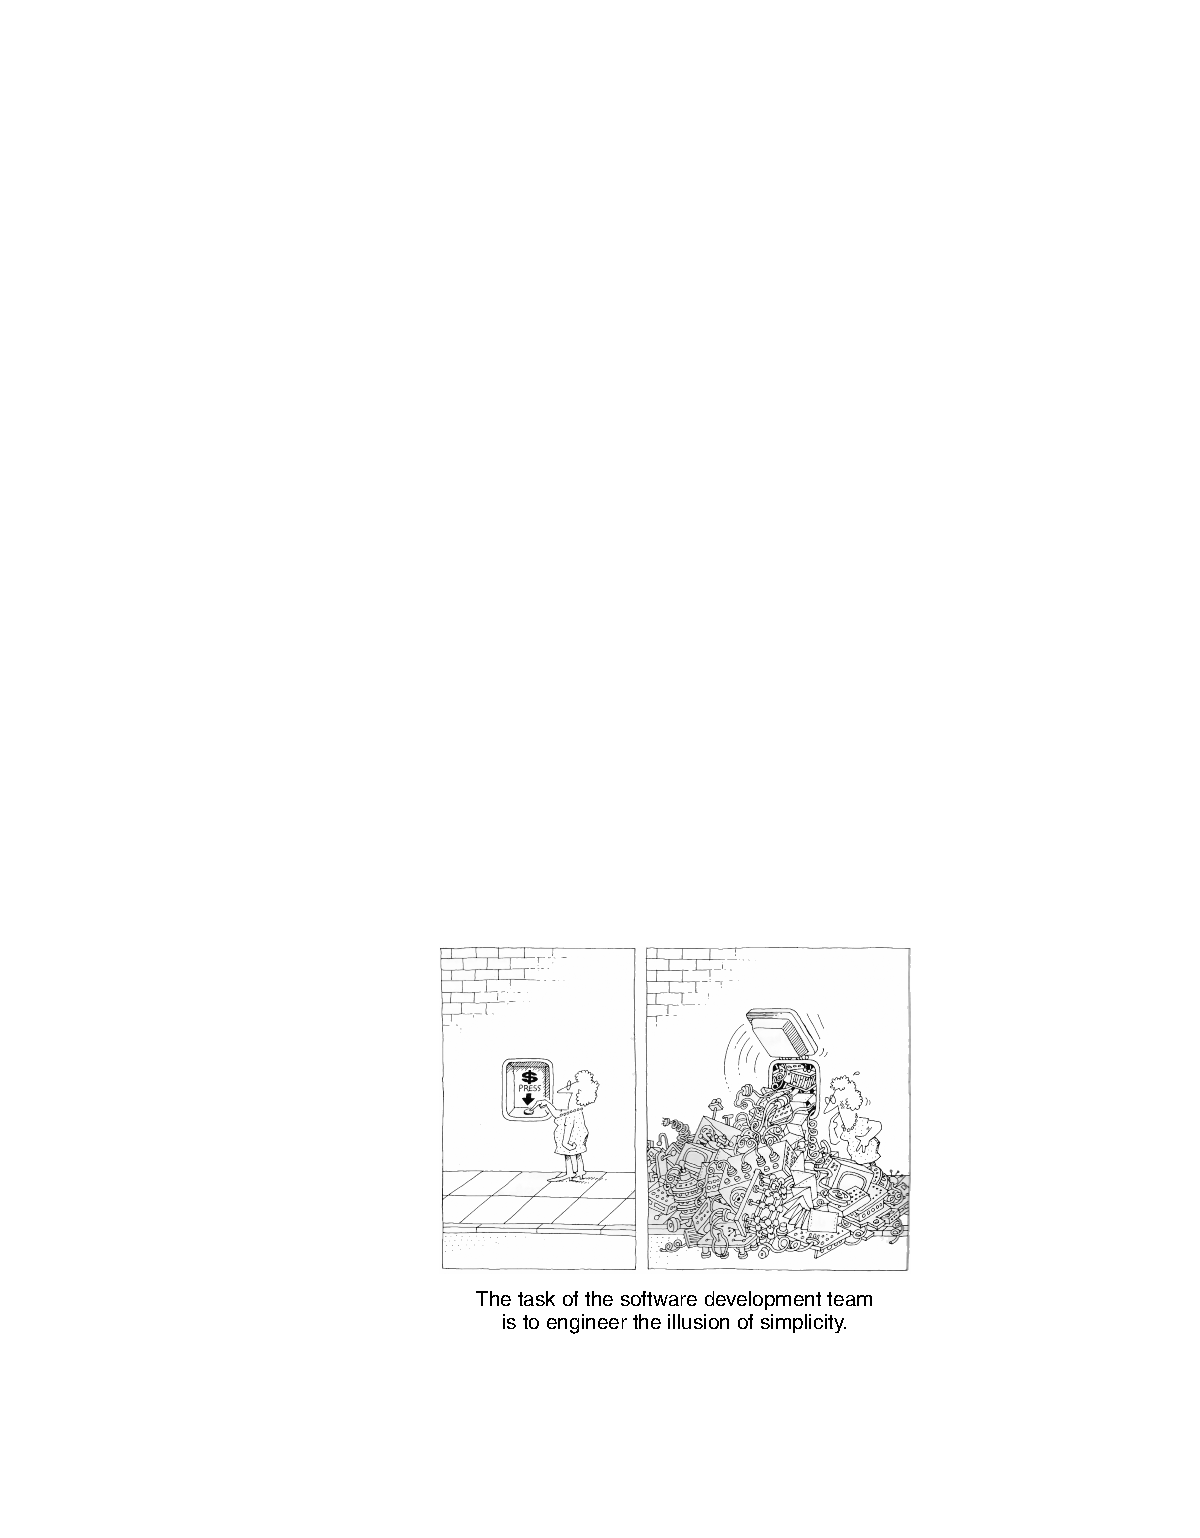
\includegraphics[width=0.8\hsize]{complexcity.pdf}
  \end{center}
\end{frame}

\begin{frame}
\frametitle{面向对象的基本思想}
\begin{enumerate}
  \item 从现实世界中客观存在的事物出发来构造系统
    \begin{itemize}
      \item 强调直接以问题域(现实世界)中的事物为中心来思考问题、认识问
        题,并根据这些事物的本质特征,把它们抽象为系统中的对象,作为系统
        的基本构成单位
      \item 这可以使系统直接映射问题域,保持问题域中事物及其
        相互关系的本来面貌
    \end{itemize}
  \item 充分运用人类日常的思维方法
    \begin{itemize}
      \item 抽象、分类、继承、聚合、封装、关联等原则
      \item 使得软件开发者能更有效地思考问题,并便于互相交流
    \end{itemize}
\end{enumerate}
\end{frame}

\begin{frame}
  \frametitle{主要特点}
  \begin{itemize}
    \item 用\textbf{\textcolor{red}{对象}}表示问题域中的事物,作为系统的基本构成单位
    \item 对象的\textbf{\textcolor{red}{属性}}和\textbf{\textcolor{red}{
      操作}}刻画了事物的静态特征和动态特征, 对外屏蔽内部细节
    \item 对象之间通过\textbf{\textcolor{red}{消息}}进行通信,以实现对象之间的动态联系
    \item 对象之间的\textcolor{red}{\textbf{继承关系}}、
      \textcolor{red}{\textbf{聚合}}关系、\textcolor{red}{\textbf{关联}}
      和\textcolor{red}{\textbf{消息}}如实地表达了问题域中事物之间实际存在的各种关系
    \item 无论系统的构成成分,还是通过这些成分之间的关系而体现的系统结
      构,都可直接地映射问题域
  \end{itemize}
\end{frame}


\subsection{形成}

\begin{frame}
  \frametitle{从认识论看面向对象方法}
  \begin{block}{软件开发: 对事物的\textcolor{red}{\textbf{认识}}和\textcolor{red}{\textbf{描述
    }}}
    \begin{itemize}
      \item 认识:对问题域找出正确的认识和理解,弄清事物的属性、行为及彼
        此之间的关系,找出解决问题的方法
      \item 描述:用一种语言把人们对问题域中事物及问题解决方案的认识描述
        出来,最终的描述必须使用计算机能理解的语言,即编程语言
      \item 编程语言的鸿沟:自然语言与机器语言之间的差距
    \end{itemize}
  \end{block}
\end{frame}

\begin{frame}
  \frametitle{语言的鸿沟}
  %\begin{center}
    %\centering\includegraphics[width=0.9\hsize]{lang-gap.pdf}
  %\end{center}
\noindent\begin{tikzpicture}
    \tikzstyle{Stage}=[rectangle, minimum height=1cm, text width=2cm, 
      align=center, fill=cyan!60];

    \node [Stage, fill=white, draw] (Problem) {问题域} ;
    \draw [thick] ([xshift=-0.5cm, yshift=-3pt]Problem.south west) --
    ([xshift=0.5cm, yshift=-3pt]Problem.south east) ;
    \node [left=1cm of Problem.south west] {自然语言} ;

    \node [below=0.2cm of Problem, text width=1pt] (Gap) {语言的鸿沟} ;

    \node [right= 1cm of Gap, align=left] (CGAP) {$\left. \begin{array}{c}
    \\
    \\
    \\
    \\
    \\
    \end{array}\right\}\mbox{语言的过渡(人)} $} ;

    \node [right= 0.05cm of Problem, align=left] {$\left.  \begin{array}{c}
      \\
      \\
    \end{array} \right\} \mbox{对问题域的认识(人)}$} ;


    \node [Stage, below=0.1cm of Gap, fill=white, draw] (Test) {计算机} ;
    \draw [thick] ([xshift=-0.5cm, yshift=3pt]Test.north west) --
    ([xshift=0.5cm, yshift=3pt]Test.north east) ;
    \node [left=1cm of Test.north west, yshift=0.1cm] {编程语言} ;
    \node [right=0.8cm of Test.north east, yshift=0.1cm] {编程(人)} ;

    \node [right= 0.05cm of Test, align=left] {$\left. \begin{array}{c}
      \\
      \\
    \end{array} \right\} \mbox{程序的理解和执行(机器)}$} ;

  \end{tikzpicture}
 
\end{frame}

\begin{frame}
  \frametitle{语言的发展使鸿沟变窄}
  \begin{columns}[c]
  \column{.4\hsize}
  \begin{block}{机器语言}
  程序的指令、数据、地址,都是由二进制的“0”和“1”构成的。离机器最近,能够
  直接地执行,然而没有丝毫形象的意义,离人类的思维最远
  \end{block}
  \column{.6\hsize}
%  \begin{center}
%    \centering\includegraphics[width=0.9\hsize]{lang-01.pdf}
%  \end{center}
\noindent\begin{tikzpicture}
    \tikzstyle{Stage}=[rectangle, minimum height=0.8cm, text width=2cm, 
      align=center, fill=cyan!60];

    \node [Stage, fill=white, draw] (Problem) {问题域} ;
    \draw [thick] ([xshift=-0.5cm, yshift=-1pt]Problem.south west) --
    ([xshift=0.5cm, yshift=-1pt]Problem.south east) ;
    \node [left=1cm of Problem.south west] {自然语言} ;

    \node [below=0.2cm of Problem] (Gap) {语言的鸿沟} ;

    \node [Stage, below=3.1cm of Gap, fill=white, draw] (Test) {计算机} ;
    \draw [thick] ([xshift=-0.5cm, yshift=1pt]Test.north west) --
    ([xshift=0.5cm, yshift=1pt]Test.north east) ;
    \node [left=1cm of Test.north west, yshift=0.1cm] {机器语言} ;

  \end{tikzpicture}
 
  \end{columns}
\end{frame}

\begin{frame}
  \frametitle{语言的发展使鸿沟变窄}
  \begin{columns}[c]
  \column{.4\hsize}
  \begin{block}{汇编语言}
    以易理解的符号表示指令、数据以及寄存器、地址等物理概念。稍稍适合人类
    的形象思维,但仍然相差很远。因为抽象层次太低,仍需考虑大量的机器细节
  \end{block}
  \column{.6\hsize}
%  \begin{center}
%    \centering\includegraphics[width=0.9\hsize]{lang-asm.pdf}
%  \end{center}
\noindent\begin{tikzpicture}
    \tikzstyle{Stage}=[rectangle, minimum height=0.8cm, text width=2cm, 
      align=center, fill=cyan!60];

    \node [Stage, fill=white, draw] (Problem) {问题域} ;
    \draw [thick] ([xshift=-0.5cm, yshift=-1pt]Problem.south west) --
    ([xshift=0.5cm, yshift=-1pt]Problem.south east) ;
    \node [left=1cm of Problem.south west] {自然语言} ;

    \node [below=0.2cm of Problem] (Gap) {语言的鸿沟} ;

    \node [Stage, below=2.1cm of Gap] (Program) {} ;
    \draw [thick] ([xshift=-0.5cm, yshift=1pt]Program.north west) --
    ([xshift=0.5cm, yshift=1pt]Program.north east) ;
    \node [left=1cm of Program.north west, yshift=0.1cm] {汇编语言} ;

    \node [Stage, below=0.1cm of Program, fill=white, draw] (Test) {计算机} ;
    \draw [thick] ([xshift=-0.5cm, yshift=1pt]Test.north west) --
    ([xshift=0.5cm, yshift=1pt]Test.north east) ;
    \node [left=1cm of Test.north west, yshift=0.1cm] {机器语言} ;

  \end{tikzpicture}
 
  \end{columns}
\end{frame}

\begin{frame}
  \frametitle{语言的发展使鸿沟变窄}
  \begin{columns}[c]
  \column{.4\hsize}
  \begin{block}{高级语言}
    隐蔽了机器细节,使用有形象意义的命名和表达式,可以联系到程序所描述的
    具体事物。特别是结构化编程语言更便于体现客观事物的结构和逻辑涵义,与
    人类的自然语言更接近,但仍有不少差距
  \end{block}
  \column{.6\hsize}
%  \begin{center}
%    \centering\includegraphics[width=0.9\hsize]{lang-high.pdf}
%  \end{center}
\noindent\begin{tikzpicture}
    \tikzstyle{Stage}=[rectangle, minimum height=0.8cm, text width=2cm, 
      align=center, fill=cyan!60];

    \node [Stage, fill=white, draw] (Problem) {问题域} ;
    \draw [thick] ([xshift=-0.5cm, yshift=-1pt]Problem.south west) --
    ([xshift=0.5cm, yshift=-1pt]Problem.south east) ;
    \node [left=1cm of Problem.south west] {自然语言} ;

    \node [below=0.2cm of Problem] (Gap) {语言的鸿沟} ;

    \node [Stage, below=1cm of Gap] (Design1) {} ;
    \draw [thick] ([xshift=-0.5cm, yshift=1pt]Design1.north west) --
    ([xshift=0.5cm, yshift=1pt]Design1.north east) ;
    \node [left=1cm of Design1.north west, yshift=0.1cm] {高级语言} ;


    \node [Stage, below=0.1cm of Design1] (Program) {} ;
    \draw [thick] ([xshift=-0.5cm, yshift=1pt]Program.north west) --
    ([xshift=0.5cm, yshift=1pt]Program.north east) ;
    \node [left=1cm of Program.north west, yshift=0.1cm] {汇编语言} ;

    \node [Stage, below=0.1cm of Program, fill=white, draw] (Test) {计算机} ;
    \draw [thick] ([xshift=-0.5cm, yshift=1pt]Test.north west) --
    ([xshift=0.5cm, yshift=1pt]Test.north east) ;
    \node [left=1cm of Test.north west, yshift=0.1cm] {机器语言} ;

  \end{tikzpicture}
  \end{columns}
\end{frame}

\begin{frame}
  \frametitle{语言的发展使鸿沟变窄}
  \begin{columns}[c]
  \column{.4\hsize}
  \begin{block}{面向对象语言}
    能比较直接地反映客观世界的本来面目,并使软件开发人员能够运用人类认识
    事物所采用的一般思维方法来进行软件开发
  \end{block}
  \column{.6\hsize}

  %\begin{center}
  %  \centering\includegraphics[width=1.0\hsize]{lang-oo.pdf}
  %\end{center}
\noindent\begin{tikzpicture}
    \tikzstyle{Stage}=[rectangle, minimum height=0.8cm, text width=2cm, 
      align=center, fill=cyan!60];

    \node [Stage, fill=white, draw] (Problem) {问题域} ;
    \draw [thick] ([xshift=-0.5cm, yshift=-1pt]Problem.south west) --
    ([xshift=0.5cm, yshift=-1pt]Problem.south east) ;
    \node [left=1cm of Problem.south west] {自然语言} ;

    \node [below=0.2cm of Problem] (Gap) {语言的鸿沟} ;

    \node [Stage, below=0.2cm of Gap] (Design0) {} ;
    \draw [thick] ([xshift=-0.5cm, yshift=1pt]Design0.north west) --
    ([xshift=0.5cm, yshift=1pt]Design0.north east) ;
    \node [left=1cm of Gap.south west, yshift=-0.1cm] {面向对象语言} ;

    \node [Stage, below=0.1cm of Design0] (Design1) {} ;
    \draw [thick] ([xshift=-0.5cm, yshift=1pt]Design1.north west) --
    ([xshift=0.5cm, yshift=1pt]Design1.north east) ;
    \node [left=1cm of Design1.north west, yshift=0.1cm] {高级语言} ;


    \node [Stage, below=0.1cm of Design1] (Program) {} ;
    \draw [thick] ([xshift=-0.5cm, yshift=1pt]Program.north west) --
    ([xshift=0.5cm, yshift=1pt]Program.north east) ;
    \node [left=1cm of Program.north west, yshift=0.1cm] {汇编语言} ;

    \node [Stage, below=0.1cm of Program, fill=white, draw] (Test) {计算机} ;
    \draw [thick] ([xshift=-0.5cm, yshift=1pt]Test.north west) --
    ([xshift=0.5cm, yshift=1pt]Test.north east) ;
    \node [left=1cm of Test.north west, yshift=0.1cm] {机器语言} ;

  \end{tikzpicture}


  \end{columns}
\end{frame}

\begin{frame}
  \frametitle{传统软件工程方法的鸿沟}
  %\begin{center}
    %\centering\includegraphics[width=0.8\hsize]{se-gap.pdf}
  %\end{center}

  \noindent\begin{tikzpicture}
    \tikzstyle{Domain}=[draw, rectangle, minimum height=0.8cm, text width=3cm, 
      align=center, thick];
    \tikzstyle{Stage}=[draw, rectangle, minimum height=0.8cm, text width=2cm, 
      align=center, fill=cyan!60, thick];

    \node [Domain] (Problem) {问题域} ;
    \node [Stage, below=0.2cm of Problem] (Analysis) {需求分析} ;
    \node [below=0.2cm of Analysis, text width=3.2cm] (Gap) {分析与设计的鸿沟} ;
    \node [Stage, below=0.2cm of Gap] (Design0) {总体设计} ;
    \node [Stage, below=0.1cm of Design0] (Design1) {详细设计} ;
    \node [Stage, below=0.1cm of Design1] (Program) {编程} ;
    \node [Stage, below=0.1cm of Program] (Test) {测试} ;
    \node [Domain, below=0.1cm of Test] (Computer) {计算机} ;

    \draw [thick] ([xshift=-1cm]Analysis.west) -- (Analysis.west) ;
    \draw [thick] (Analysis.east) -- ([xshift=1cm]Analysis.east) ;
    \draw [thick] ([xshift=-1cm]Program.west) -- (Program.west) ;
    \draw [thick] (Program.east) -- ([xshift=1cm]Program.east) ;
    \node [left=1.2cm of Analysis] {自然语言} ;
    \node [left=1.2cm of Program] {编程语言} ;

    \node[cloud callout, draw, thick, cloud puffs=10, aspect=1.6, 
      cloud puff arc=120, align=center, right=1.5cm of Design1, callout
      pointer segments=3, 
      callout absolute pointer=(Gap.east)] {分析与设计\\概念及表示法\\的不一致};
  \end{tikzpicture}

\end{frame}

\begin{frame}
  \frametitle{面向对象的软件工程方法}
  %\begin{center}
    %\centering\includegraphics[width=0.7\hsize]{oose.pdf}
  %\end{center}
\noindent\begin{tikzpicture}
    \tikzstyle{Domain}=[draw, rectangle, minimum height=0.8cm, text width=3cm, 
      align=center, thick];
    \tikzstyle{Stage}=[draw, rectangle, minimum height=0.8cm, text width=2cm, 
      align=center, fill=cyan!60];

    \node [Domain] (Problem) {问题域} ;
    \node [Stage, below=0.2cm of Problem] (Analysis) {OOA} ;
    \node [Stage, below=0.0cm of Analysis] (Design) {OOD} ;
    \node [Stage, below=0.0cm of Design] (Program) {OOP} ;
    \node [Stage, below=0.0cm of Program] (Test) {OOT} ;
    \node [Domain, below=0.2cm of Test] (Computer) {计算机} ;

    \draw [thick] ([xshift=-1cm]Analysis.west) -- (Analysis.west) ;
    \draw [thick] (Analysis.east) -- ([xshift=1cm]Analysis.east) ;
    \draw [thick] ([xshift=-1cm]Program.west) -- (Program.west) ;
    \draw [thick] (Program.east) -- ([xshift=1cm]Program.east) ;
    \node [left=1.2cm of Analysis] {自然语言} ;
    \node [left=1.2cm of Program] {编程语言} ;

  \end{tikzpicture}


\end{frame}

\section{基本概念}

\begin{frame}
  \frametitle{面向对象基本概念与原则集}
  \begin{itemize}
    \item 对象,类
    \item 属性,操作
    \item 封装
    \item 继承,一般-特殊结构
    \item 聚合,整体-部分结构
    \item 关联
    \item 消息
    \item 多态
    \item 持久对象,主动对象
    \item \ldots
  \end{itemize}
\end{frame}

\subsection{核心}

\begin{frame}
  \frametitle{对象: object}
  \only<1> {
  \begin{block}{现实中的对象}
    \textbf{\textcolor{red}{对象}}是现实世界中某个实际存在的事物,它可以
    是有形的,比如一辆汽车,也可以是无形的,比如一项计划 \\
    对象是构成世界的一个独立单位,它具有自己的静态特征和动态特征
  \end{block}

  \begin{center}
    \centering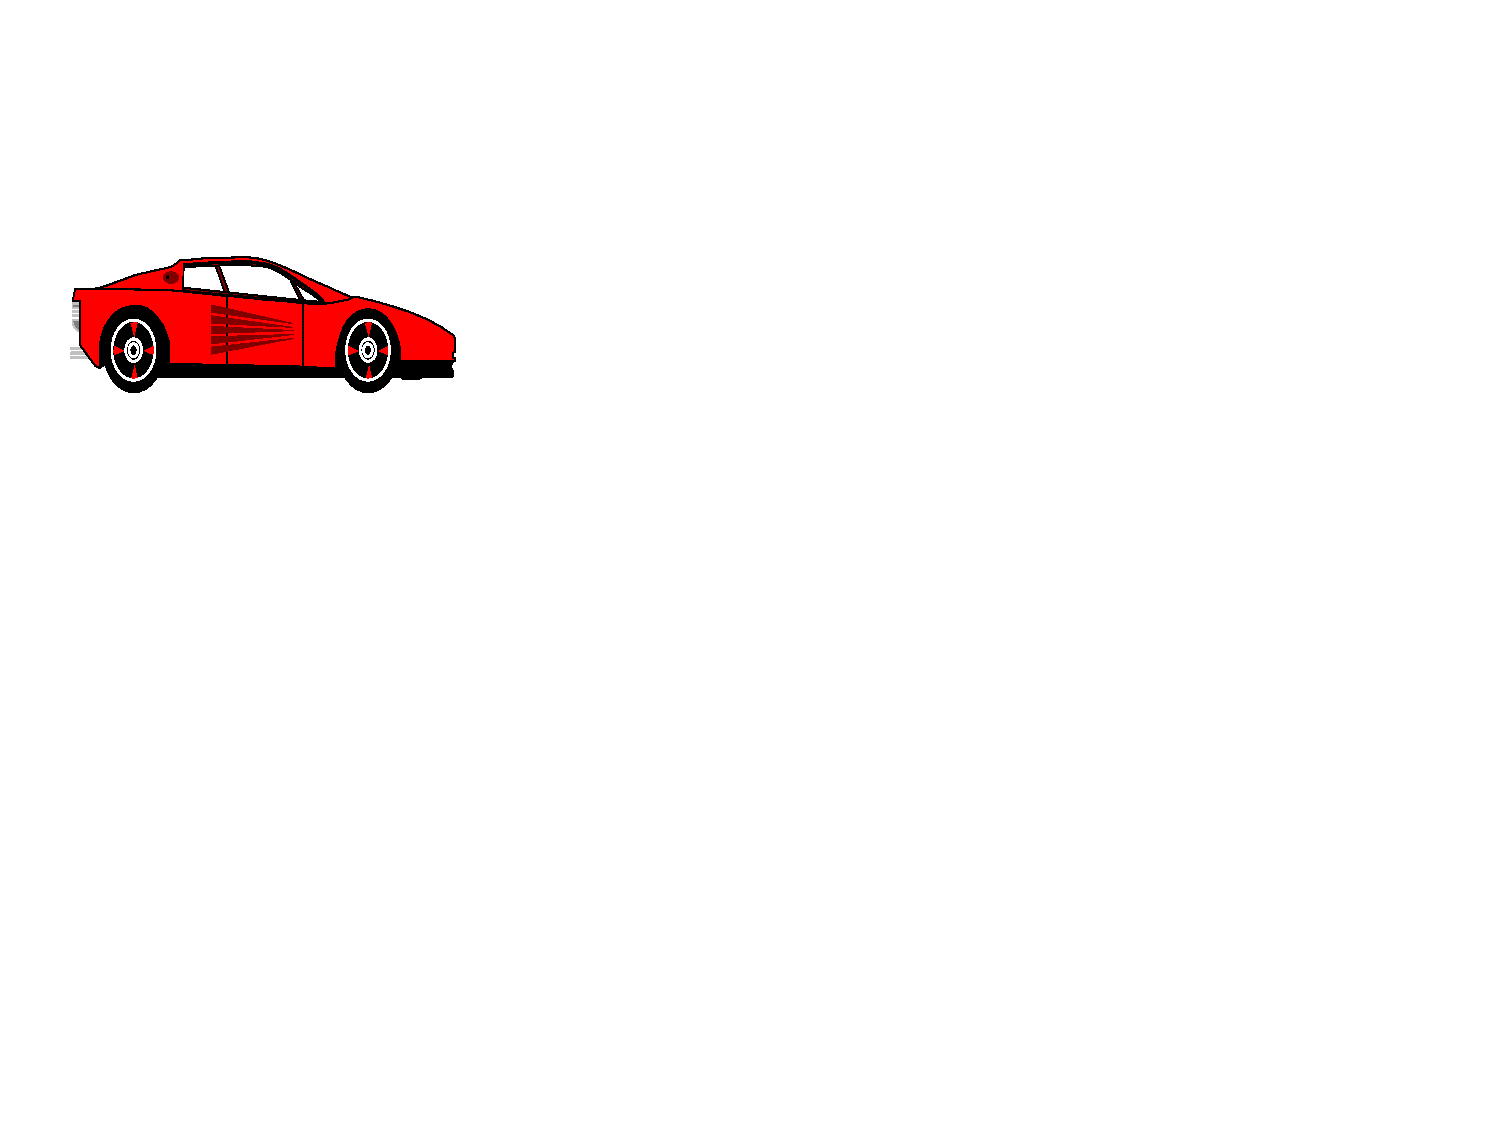
\includegraphics[width=0.4\hsize]{car.pdf}
  \end{center}
}

\only<2> {
  \begin{block}{软件中的对象}
    \textbf{\textcolor{red}{对象}}
    是系统中用来描述客观事物的一个实体,它是构成系统的一个基本单位。\\
    对象由一组\textbf{\textcolor{red}{属性}}和施加于这些属性的一组
    \textbf{\textcolor{red}{操作}}构成
  \end{block}
  \begin{center}
    \begin{minipage}[c]{.25\textwidth}
    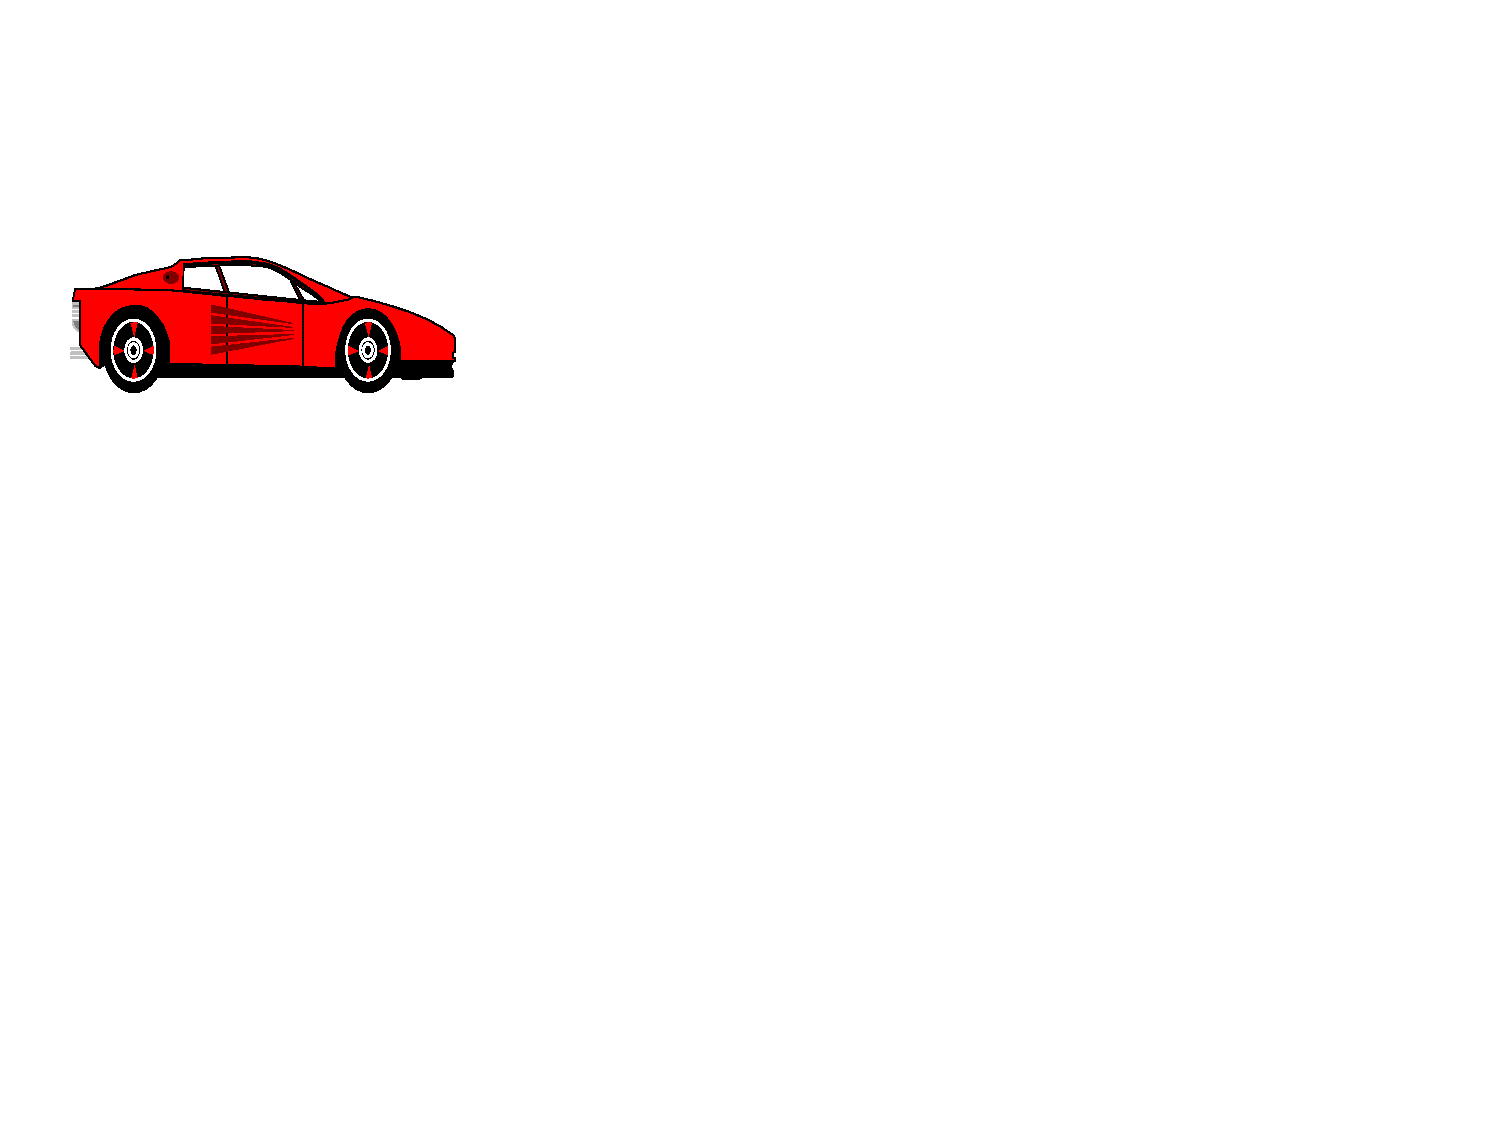
\includegraphics[width=0.9\hsize]{car.pdf}\hfill
    \end{minipage}%
    \begin{minipage}[c]{.2\textwidth}
      \centering$\Longrightarrow$
    \end{minipage}%
    \begin{minipage}[c]{.25\textwidth}

    %\centering\includegraphics[width=0.6\hsize]{object.pdf}
      \begin{tikzpicture}
        \umlclass[fill=white]{对象标识}{属性}{操作}
        \node [above=0.1cm of 对象标识, red] {对象} ;
      \end{tikzpicture}

    \end{minipage}
  \end{center}
}
\end{frame}

\begin{frame}
  \frametitle{对象的属性、操作、标识}
  \begin{block}{属性: attribute}
    属性是用来描述对象静态特征的一个数据项
  \end{block}
  \begin{block}{操作: operation}
    操作是用来描述对象动态特征的一个动作序列
  \end{block}
  \begin{block}{标识: identification}
    对象标识就是对象的名字,有“外部标识”和“内部标识”之分
  \end{block}
\end{frame}
 
\begin{frame}
  \frametitle{封装}
  \begin{block}{封装: encapsulation}
    把对象的属性和操作结合成一个独立的系统单位,并尽可能隐蔽对象的内部细
    节
  \end{block}
  \begin{center}
    \centering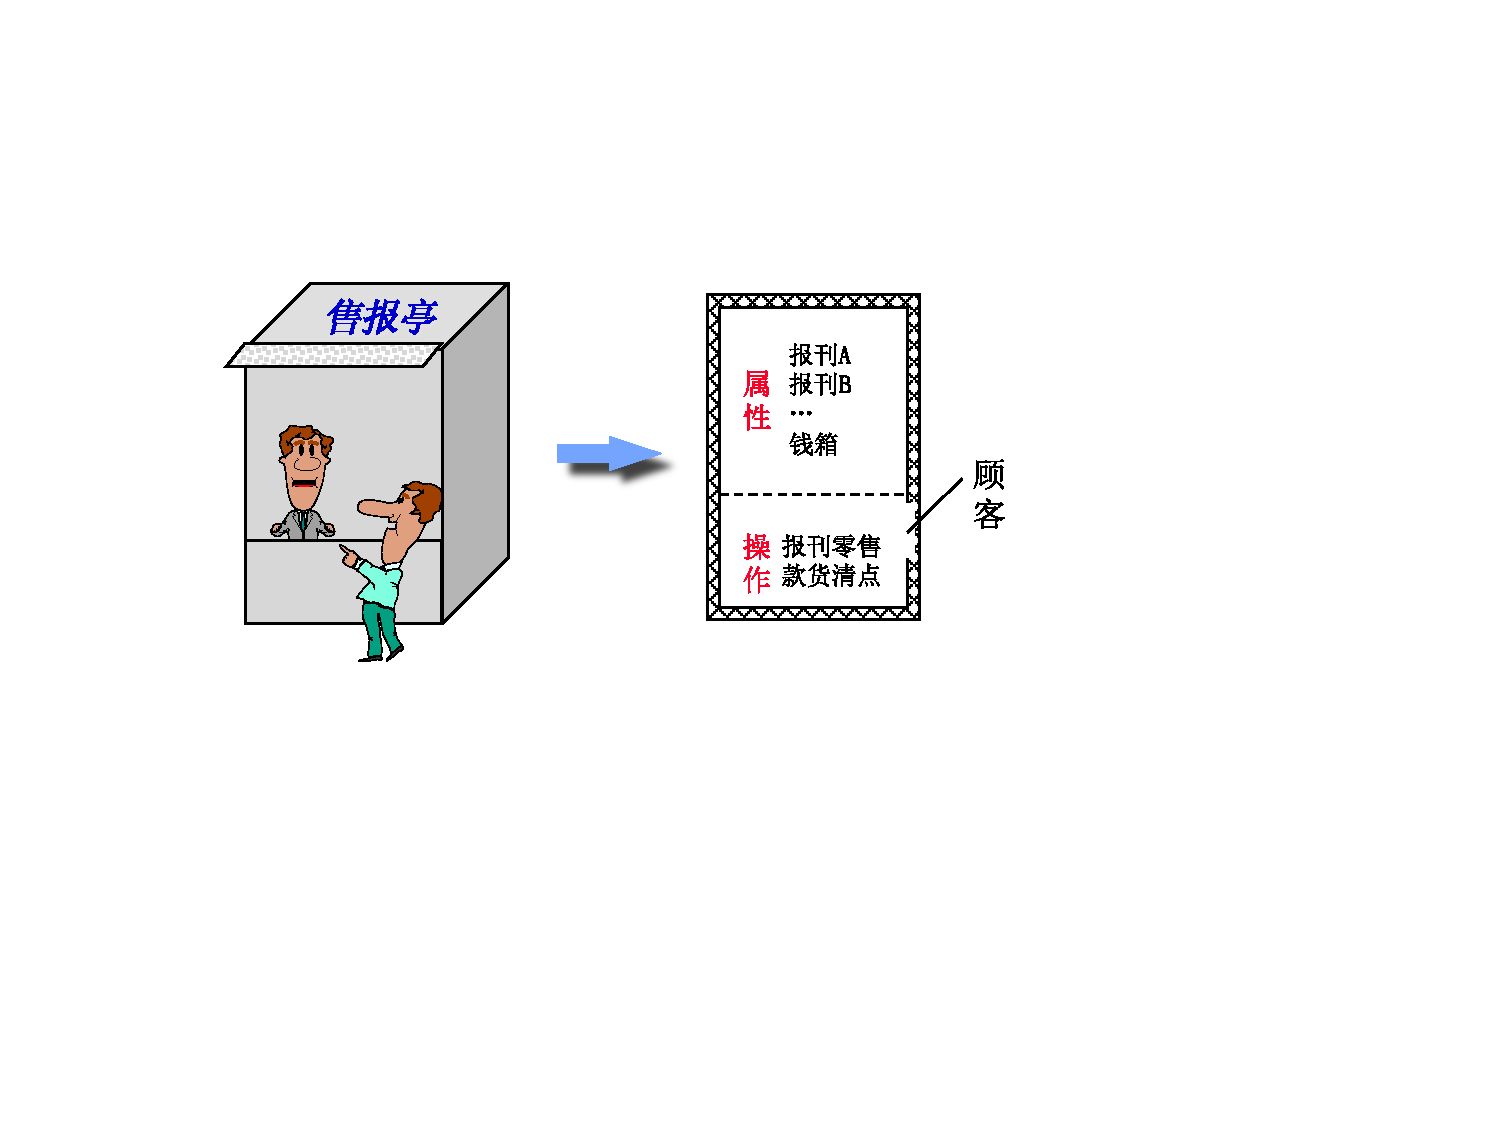
\includegraphics[width=0.6\hsize]{seller.pdf}
  \end{center}
\end{frame}


\begin{frame}
  \frametitle{封装的意义}
  \begin{itemize}
    \item 使对象能够集中而完整地描述并对应一个具体的事物
    \item 体现了事物的相对独立性,使对象外部不能随意存取对象的内部数据,避免
      了外部错误对它的“交叉感染”
    \item 对象的内部的修改对外部的影响很小,减少了修改引起的“波动效应”
  \end{itemize}
\end{frame}

\begin{frame}
  \frametitle{封装的问题}
  \begin{itemize}
    \item 编程的麻烦
    \item 执行效率的损失
  \end{itemize}
  \begin{block}{解决办法}
    不强调严格封装, 实行可见性控制 \\
    常见于混合型OOPL, 如C++
  \end{block}
\end{frame}

\begin{frame}
  \frametitle{抽象与分类}
  \begin{block}{抽象}
    忽略事物的非本质特征,只注意那些与当前目标有关的本质特征,从而找出事
    物的共性,叫做抽象 \\
    抽象是形成概念的基本手段
  \end{block}
  \begin{block}{分类}
    把具有共同性质的事物划分为一类,叫做分类
  \end{block}
\end{frame}

\begin{frame}
  \frametitle{类与对象}
  \begin{columns}[c]
  \column{.6\hsize}
  \begin{block}{类: class}
    类是具有相同属性和操作的一组对象的集合,它为属于该类的全部对象提供了
    统一的\textbf{\textcolor{red}{抽象}}描述,其内部包括属性和操作两个主
    要部分\\
    在程序设计中,类的作用是用来创建对象,对象是类的一个实例
  \end{block}
  \column{.4\hsize}

%  \begin{center}
%    \centering\includegraphics[width=0.9\hsize]{abstract.pdf}
%  \end{center}

\begin{tikzpicture}
\foreach \x/\y in {1/0, 1.5/0.2, 2/0.4, 2.5/0.6, 3/0.8, 3.5/1, 4/1.2} {
  \node [draw, rectangle, thick, fill=white] at (\x, \y) {对象} ;
}

\node at (2.5,2) [single arrow, draw, rotate=90]{抽象};

\umlclass[x=2.5, y=4.5, fill=white]{类名}{属性}{操作}

\end{tikzpicture}

  \end{columns}
\end{frame}

\begin{frame}
  \frametitle{抽象与分类的不同层次}
  \begin{itemize}
    \item 较多地忽略事物之间的差别可得到较一般的类
    \item 较多地注意事物之间的差别可得到较特殊的类
  \end{itemize}
  %\begin{center}
    %\centering\includegraphics[width=0.4\hsize]{transport.pdf}
  %\end{center}
\vspace*{2ex}

\centering\begin{tikzpicture}
\tikzumlset{fill class=white}
\umlsimpleclass{运输工具}
\umlsimpleclass[y=-1.5]{车辆}
\umlsimpleclass[x=-2, y=-1.5]{轮船}
\umlsimpleclass[x=2, y=-1.5]{飞机}
\umlsimpleclass[x=-1, y=-3]{火车}
\umlsimpleclass[x=1, y=-3]{汽车}
\umlsimpleclass[x=0, y=-4.5]{卡车}
\umlsimpleclass[x=2, y=-4.5]{轿车}
\umlinherit[geometry=|-|]{轮船}{运输工具}
\umlinherit[geometry=|-|]{飞机}{运输工具}
\umlinherit[geometry=|-|]{火车}{车辆}
\umlinherit[geometry=|-|]{汽车}{车辆}
\umlinherit[geometry=|-|]{卡车}{汽车}
\umlinherit[geometry=|-|]{轿车}{汽车}
\umlinherit{车辆}{运输工具}
\end{tikzpicture}
\end{frame}

\begin{frame}
  \frametitle{一般类与特殊类}
  \begin{definition}
    如果类A具有类B的全部属性和全部操作,而且具有自己特有的某些属性或操作
    ,则A叫做B的\textbf{\textcolor{red}{特殊类}},B叫做A的
    \textbf{\textcolor{red}{一般类}}\\
    一般类与特殊类又称\textbf{\textcolor{red}{父类}}与
    \textbf{\textcolor{red}{子类}}
  \end{definition}

  \begin{definition}
    如果类A的全部对象都是类B的对象,而且类B中存在不属于类A的对象,则A是B
    的特殊类,B是A的一般类
  \end{definition}
\end{frame}

\begin{frame}
  \frametitle{继承}
  \begin{block}{继承: inheritance}
    特殊类拥有其一般类的全部属性与操作,称作特殊类对一般类的继承
    \begin{itemize} 
      \item 继承意味着\textbf{\textcolor{red}{自动地拥有}},或曰
    \textbf{\textcolor{red}{隐含地复制}},由继承机制保证
      \item 继承简化了人们对事物的认识和描述,在一定程度上有益于
        \textbf{\textcolor{red}{软件复用}}
    \item 避免过度使用继承
    \end{itemize}
  \end{block}
\end{frame}

\begin{frame}
  \frametitle{继承关系的语义}
  \begin{columns}[c]
  \column{.5\hsize}
  \begin{block}{一般 - 特殊结构}
    由一组具有继承关系的类所组成的结构,其以类为
    结点、以继承关系为边形成连通的有向图 \\
    继承关系的语义:\textbf{\textcolor{red}{is a}}, 或
\textbf{\textcolor{red}{is a kind of}}
  \end{block}
  \column{.5\hsize}
  %\begin{center}
    %\centering\includegraphics[width=0.9\hsize]{soldier.pdf}
  %\end{center}
  \begin{tikzpicture}
    \tikzumlset{fill class=white}
    \umlsimpleclass{军人}
    \umlsimpleclass[x=-1, y=-2]{军官}
    \umlsimpleclass[x=1, y=-2]{士兵}
    \umlsimpleclass[x=-0.5, y=-4]{义务兵}
    \umlsimpleclass[x=2.5, y=-4]{志愿兵}

    \umlinherit[geometry=|-|]{军官}{军人}
    \umlinherit[geometry=|-|]{士兵}{军人}
    \umlinherit[geometry=|-|]{义务兵}{士兵}
    \umlinherit[geometry=|-|]{志愿兵}{士兵}
  \end{tikzpicture}
  \end{columns}
\end{frame}

\begin{frame}
  \frametitle{多继承: 子类具有多个父类}
  %\begin{center}
    %\centering\includegraphics[width=0.3\hsize]{m-inheritence.pdf}
  %\end{center}
\centering\scalebox{0.8}{
  \begin{tikzpicture}
    \tikzumlset{fill class=white}

    \umlclass{人员}{姓名}{}
    \umlclass[x=-2, y=-3.5]{研究生}{学号\\班级\\专业}{}
    \umlclass[x=2, y=-3.5]{教职工}{职称\\专业}{}
    \umlclass[y=-7]{在职研究生}{在职单位}{}

    \umlinherit[geometry=|-|, arm1=1.8cm]{研究生}{人员}
    \umlinherit[geometry=|-|, arm1=1.8cm]{教职工}{人员}
    \umlinherit[geometry=|-|, arm1=1.5cm]{在职研究生}{研究生}
    \umlinherit[geometry=|-|, arm1=1.5cm]{在职研究生}{教职工}
  \end{tikzpicture}
}
\end{frame}

\begin{frame}
\frametitle{聚合}
\begin{block}{聚合: aggregation}
是两个类之间的一个二元关系,它表示一个类的对象实例以另一个类的对象实例作为其组成部分 \\
聚合刻画了现实事物之间的\textbf{\textcolor{red}{构成}}关系或者\textbf{\textcolor{red}{拥有}}关系 \\
聚合关系的语义:\textbf{\textcolor{red}{has a}} 或 \textbf{\textcolor{red}{is a part of}}
\end{block}
\end{frame}

\begin{frame}
\frametitle{两种聚合方式}
\only<1> {
\begin{block}{ 紧密、固定的聚合关系}
又称为组合关系(composition), 如汽车与发动机, 常实现为嵌套对象
\end{block}

\vspace*{4ex}
\centering\begin{tikzpicture}
    %\node [draw, rectangle, rounded corners, thick, minimum width=4cm,
    %minimum height=3cm] {整体对象} ;
    \node [draw, rectangle, rounded corners, thick] (Whole) {
      \begin{minipage}[t][2cm]{5cm} \centering 整体对象\end{minipage}} ;

      \node [draw, rectangle, rounded corners, thick, right= 0.3cm of
      Whole.west, yshift=-0.2cm] (Part1) {部分对象} ;
      \node [draw, rectangle, rounded corners, thick, left= 0.3cm of
      Whole.east, yshift=-0.2cm] (Part1) {部分对象} ;
  \end{tikzpicture}

}

\only<2> {
\begin{block}{松散、灵活的聚合关系}
例如公司与法律顾问, 常实现为对象指针\\
\end{block}

\vspace*{4ex}
  \begin{tikzpicture}
    \node [draw, rectangle, rounded corners, thick, minimum width=1.5cm,
    text width=2ex] (Whole1) {整体对象} ;

    \node [scale=0.5, minimum size=1pt, fill=black, circle, left=0.1cm
    of Whole1.east, yshift=0.8cm ] (Ref11) {} ;
    \node [scale=0.5, minimum size=1pt, fill=black, circle, left=0.1cm
    of Whole1.east, yshift=-0.8cm ] (Ref12) {} ;

    \node [draw, rectangle, rounded corners, thick, right= 1.5cm of
    Whole1, yshift=0.8cm] (Part1) {部分对象} ;
    \node [draw, rectangle, rounded corners, thick, right= 1.5cm of
    Whole1, yshift=-0.8cm] (Part2) {部分对象} ;

    \node [draw, rectangle, rounded corners, thick, minimum width=1.5cm,
    text width=2ex, right=5cm of Whole1] (Whole2) {整体对象} ;
    \node [scale=0.5, minimum size=1pt, fill=black, circle, right=0.1cm
    of Whole2.west] (Ref21) {} ;

    \draw [thick, ->, red] (Ref11) to [bend left] (Part1.west) ;
    \draw [thick, ->, red] (Ref12) to [bend right] (Part2.west) ;
    \draw [thick, ->, red] (Ref21) to [bend left] (Part2.east) ;

  \end{tikzpicture}

}

\end{frame}

\begin{frame}
\frametitle{整体-部分结构}
\begin{block}{ 整体-部分结构}
聚合关系又称整体-部分关系。由一组具有聚合关系的类所形成的结构称为整体-部分结构。它是一个以类为结点,以聚合关系为边的连通有向图
\end{block}

\vspace*{2ex}
\scalebox{0.9}{
\begin{tikzpicture}
  \tikzumlset{fill class=white}
  \umlsimpleclass{汽车}
  \umlsimpleclass[x=-2, y=-1.5]{发动机}
  \umlsimpleclass[x=2, y=-1.5]{车身}
  \umlsimpleclass[x=-2, y=-3.5]{气缸}

  \umlsimpleclass[x=5]{公司}
  \umlsimpleclass[x=5, y=-3]{法律顾问}

  \umlcompo[mult1=1, mult2=1]{汽车}{发动机}
  \umlcompo[mult1=1, mult2=1]{汽车}{车身}
  \umlcompo[mult1=1, mult2=1..*]{发动机}{气缸}

  \umlaggreg[mult1=0..*, mult2=0..*]{公司}{法律顾问}
\end{tikzpicture}
}
\end{frame}

\begin{frame}
\frametitle{关联}
\begin{block}{关联: association}
两个或者多个类上的一个关系(即这些类的对象实例集合的笛卡儿积的一个子集合),其中的元素提供了被开发系统的应用领域中一组有意义的信息  \\
二元关联, 多元关联
\end{block}

\vspace*{2ex}

\begin{tikzpicture}
  \tikzumlset{fill class=white}
  \umlclass{教师}{}{}
  \umlclass[x=4]{学生}{}{}
  \umlassoc[mult1=1, mult2=*, arg=指导论文, pos=0.6]{教师}{学生}

  \umlclass[x=7]{城市}{}{}
  \umlassoc[arg=有航线, mult1=*, mult2=*, pos=0.5, recursive=-90|0|3cm]{城市}{城市}

\end{tikzpicture}
\end{frame}

\begin{frame}
\frametitle{二元关联: binary association}
假定 $A$ 和 $B$ 是系统中两个类的对象实例集合

$ A = \{a_1, a_2, \mbox{\ldots}, a_m\} $, 
$ B = \{b_1, b_2, \mbox{\ldots}, b_n\} $

$A$和$B$的笛卡尔积(Cartesian product) $A\times B$ 是一个集合,
其元素是$m \times n$个有序对,这些有序对的第一个元素为$A$集合中的元素,另
一个为集合$B$中的元素。形式化表示为
\[A\times B=\{(a,b):a\in A\mbox{~且~}b\in B\}\]

该集合的元素任意组合, 可形成 $2^{m \times n}$种集合, 每种集合都是 $A$ 和 $B$ 之间的一个关系. 实际系统中只有有意义的关系才可能定义为关联

\end{frame}

\begin{frame}
\frametitle{关联关系示例}
\begin{example}
在一个教学管理系统中有教师、学生、教务员课程等类。系统中需要表明每一门课程由哪位教师承担、有哪些学生选修。该系统的教务员要为学生做注册、登记成绩等工作,但是不需要区别是哪个教务员为哪个学生做的 
\end{example}

\vspace*{2ex}

\begin{tikzpicture}
  \tikzumlset{fill class=white}
  \umlsimpleclass{教师}
  \umlsimpleclass[x=4]{课程}
  \umlsimpleclass[x=8]{学生}
  \umlsimpleclass[x=6, y=-2]{教务员}

  \umlassoc[arg1=1, arg2=*]{教师}{课程}
  \umlassoc[arg1=*, arg2=*]{课程}{学生}

  \umldep[stereo=call]{教务员}{课程}
  \umldep[stereo=call]{教务员}{学生}
\end{tikzpicture}

\end{frame}

\begin{frame}
\frametitle{关联的多重性}
\begin{block}{多重性: multiplicity}
关联的多重性标识参加关联的对象实例在数量上所遵守的约束,有一对一、一对多、多对一、多对多等不同情况
\end{block}
数量示例: \\
\begin{tabular}{ll}
0..1 & 表示0或1个对象 \\
0..* 或 * & 表示0到多个对象 \\
1..25 & 表示1到25个对象 \\
10 & 表示 10个对象
\end{tabular}
\end{frame}

\begin{frame}
\frametitle{关联 vs 聚合}
\begin{itemize}
  \item 有时可认为聚合是一种特殊的关联关系,尤其是松散聚合
    \begin{itemize}
      \item 松散聚合和关联关系在程序设计技术上是一样的
    \end{itemize}
  \item 松散聚合有明显的 \textbf{整体-部分}语义
  \item 具体应用中采用何种结构取决于应用语义
\end{itemize}
\end{frame}

\begin{frame}
  \frametitle{消息}
  \begin{block}{消息: message}
    消息是向对象发出的服务请求.  目前在大部分面向对象的编程语言中,消息其实就是函数或过程调用(通常是同步调用)
    \begin{itemize}
      \item 消息协议: 对操作(函数)具有的消息格式的描述
      \item 函数调用只是实现消息的方式之一, 常见于顺序系统
    \end{itemize}
  \end{block}

  \begin{block}{消息的一般定义}
    消息是对象之间在一次交互中所传送的信息
  \end{block}
\end{frame}

\begin{frame}
  \frametitle{消息和关联是独立的}
  一种误解:认为在任何两个类之间只有存在关联才可能存在消息。
  实际上,关联和消息是两个截然不同的概念,二者是相互独立的 \\[2ex]

\begin{tikzpicture}
  \tikzumlset{fill class=white}
  \umlsimpleclass{教师}
  \umlsimpleclass[x=4]{课程}
  \umlsimpleclass[x=8]{学生}
  \umlsimpleclass[x=6, y=-2]{教务员}

  \umlassoc[arg1=1, arg2=*, anchor1=10, anchor2=170]{教师}{课程}
  \umlassoc[arg1=*, arg2=*]{课程}{学生}

  \umldep[stereo=call, anchor1=-10, anchor2=190]{教师}{课程}
  \umldep[stereo=call]{教务员}{课程}
  \umldep[stereo=call]{教务员}{学生}
\end{tikzpicture}
\end{frame}

\begin{frame}
  \frametitle{多态}

  \begin{block}{多态: polymorphism}
    多态是指同一个命名可具有不同的语义。OO方法中,常指在一般类中定义的属
    性或操作被特殊类继承之后,可以具有不同的数据类型或表现出不同的行为
  \end{block}

  \centering\scalebox{0.8}{
  \begin{tikzpicture}
    \tikzumlset{fill class=white}
    \umlclass{Animal}{}{talk():String}
    \umlclass[x=-2, y=-3]{Cat}{}{talk():String}
    \umlclass[x=2, y=-3]{Dog}{}{talk():String}
    \umlinherit{Cat}{Animal}
    \umlinherit{Dog}{Animal}
  \end{tikzpicture}
}
\end{frame}

\begin{frame}
  \frametitle{多态的实现机制}
    \begin{itemize}
      \item 重写(override)——在特殊类中对继承来的属性或操作重新定义其实现
      \item 动态绑定(dynamic binding)——有时也称为延迟绑定(late
        binding),在运行时根据对象接收的消息动态地确定要
    连接哪一段操作代码
  \item 类属(generic)——操作参量的类型可以是参数化的
\end{itemize}
\end{frame}

\begin{frame}[fragile]
  \frametitle{多态实现机制示例: 重写与动态绑定}

\renewcommand{\baselinestretch}{1.1}
\begin{Verbatim}[fontsize=\footnotesize]
abstract class Animal {
    abstract String talk();
}
class Cat extends Animal {
    String talk() { return "Meow!"; }
}
class Dog extends Animal {
    String talk() { return "Woof!"; }
}
void lets_hear(Animal a) {
    println(a.talk());
}
void main() {
    lets_hear(new Cat());
    lets_hear(new Dog());
}
\end{Verbatim}

\end{frame}

\begin{frame}[fragile]
  \frametitle{多态实现机制示例: 类属}

\begin{Verbatim}
class List<T> {
    class Node<T> {
        T elem;
        Node<T> next;
    }
    Node<T> head;
    int length() { ... }
}
 
List<B> map(Func<A,B> f, List<A> xs) {
    ...
}
\end{Verbatim}

\end{frame}


\subsection{其他}

\begin{frame}
  \frametitle{持久对象}
\begin{block}{持久对象: persistent object}
生存期可以超越程序的执行时间而长期存在的对象
\end{block}
\begin{itemize}
\item 现实需求: 把对象及其属性信息长期保存, 在程序启动时可重建对象, 实现很繁琐
\item 实现途径: 支持持久对象的OOPL,OO-DBMS,支持O-R映射的持久存储框架等
\end{itemize}
\end{frame}

\begin{frame}
  \frametitle{主动对象}
\begin{block}{主动对象: active object}
至少有一个操作不需要接收消息就能主动执行的对象\\
主动操作: 主动对象中能够主动执行的操作
\end{block}
\begin{itemize}
\item 现实需求: 描述具有主动行为的事物,并发执行的多个控制流
\item 实现途径: 实现阶段主要通过进程或线程等支撑系统的机制实现
\end{itemize}
\end{frame}

\begin{frame}
\frametitle{面向对象是软件方法学的返朴归真}
软件科学的发展历程中出现过许多“面向”: 面向机器、面向代数、
面向过程、 面向数据、 面向人、 面向文件、 面向信息、 面向应用、 
面向功能、 面向数据流、\ldots

\textcolor{red}{\textbf{面向对象}} 使
软件开发从过分专业化的方法、规则和技巧中回到了客观世界,回到了人们的日常思维,是软件理论的返朴归真

\end{frame}


\section{历史现状}

\subsection{起源}

\begin{frame}
\frametitle{哲学基础}
\begin{block}{软件开发: 对事物的认识和描述}
用计算机语言将人们关心的现实世界映射到计算机世界 \\
形而上学$\Longrightarrow$ 认识论 $\Longrightarrow$ 方法论
\end{block}

维特根斯坦(Ludwig Wittgenstein)于1921年发表的《逻辑哲学论》(又译《名理论》,英语、拉丁语:Tractatus
Logico-philosophicus,德语:Logisch-Philosophische Abhandlung), 有人认为是面
向对象思想的哲学来源

\end{frame}

\begin{comment}
在八十年前面向对象是作为认识世界的哲学思想被提出的,这种思想由本世纪最伟
大的哲学家维特根斯坦阐述于1922出版的《逻辑哲学论》(《
Logisch-Philosophische Abhandlung》)这一著作中。维特根斯坦认为:世界是
由简单的基本的对象构成的(《逻辑哲学论》2.021 对象构成世界的实体,因此它
们不能是复合的),这就是面向对象设计的基石。

  维特根斯坦在《逻辑哲学论》 一书中提出了如下思想:
  世界可以分解为事实 ( The world divides into facts.)
  事实是由原子事实(atomic facts)组成的。
  一个原子事实是多个对象(objects)的组合。
  对象是简单的(基本的) The Object is simple。
  对象形成了世界的基础。

  面向对象的两大核心概念是:“对象”与“类”。“一切皆是对象”是由朴素原子论而
  来的。“万物皆有类属”就是由亚里斯多德的形而上学来的。

在正文中有七个主要命题。它们是:

    世界是所有发生的事物。
    发生的事物(事实)是原子性事态的存在。
    事实的逻辑图像是思想。
    思想是有意义的命题。
    命题是基本命题的真值函数。
    命题的一般形式是真值函数的一般形式,它是: [{\bar p},{\bar \xi },N({\bar \xi })]。这也是命题的一般形式。
    对于不可说的东西我们必须保持沉默。

\end{comment}

\begin{frame}
\frametitle{逻辑哲学论的7个论题}
\begin{enumerate}

\item The world is everything that is the case.
\item What is the case (a fact) is the existence of states of affairs.
\item A logical picture of facts is a thought.
\item A thought is a proposition with a sense.
\item A proposition is a truth-function of elementary propositions. (An elementary proposition is a truth-function of itself.)
\item The general form of a proposition is the general form of a truth function, which is: $[\bar p,\bar\xi, N(\bar\xi)]$. This is the general form of a proposition.
\item Whereof one cannot speak, thereof one must be silent.
\end{enumerate}
\end{frame}

\begin{frame}
  \frametitle{逻辑哲学论中的对象思想}

\begin{itemize}
\item 世界是所有事实(fact, or case)的总和
\item 事实是原子事实(atomic facts)的存在
\item 原子事实由若干对象(objects)组成
\item 对象是简单的 
\item 对象形成了世界的基础
\item 对象构成了主观世界和客观世界的共同之处--模式(form)
\end{itemize}

\end{frame}

\subsection{发展}

\begin{frame}
\frametitle{雏形阶段}
\begin{itemize}
\item Simula67: 1960s, 首次引入类的概念和继承机制
\item 并发Pascal, Ada和Modula-2等: 1970s, 抽象数据类型, 封装
\item Flex: Alan Kay的首次尝试, 借鉴了类、对象、继承等概念
\item Smalltalk-72: 1972, Alan Kay在Palo Alto的再次尝试, 
吸收Simula67、CLU、LISP、LOGO等语言的若干思想, 
首次正式使用“面向对象”术语, 支持继承与封装, 标志着面向对象程序设计方法的正式形成
\end{itemize}
\end{frame}

\begin{frame}
\frametitle{完善阶段}
\begin{itemize}
\item Smalltalk-72, 76, 78, 80: Smalltalk-80被认为是面向对象语言发展史上最重要的里程碑,绝大部分面向对象基本概念和支持机制都已具备,是第一个完善的、能实际应用的面向对象语言
\item 但Smalltalk应用并不够广泛,除了新方法学不易被接受和商品化过程较晚的因素,
其纯面向对象的宗旨使许多开发人员感到不便
\end{itemize}
\end{frame}

\begin{frame}
\frametitle{繁荣阶段}
\begin{itemize}
\item 自80年代中期到90年代,大批较实用的OOPL涌现,例如 C++、Objective-C、Java等
\item 混合型OO语言是在传统的过程式语言基础上增加OO语言成分,
在实用性方面相比纯OO语言具有更大的优势
\item 此时的纯OO语言也比较重视实用性
\item GUI的推动
\end{itemize}
\end{frame}

\begin{frame}
\frametitle{发展到软件生存周期前期阶段}
\begin{itemize}
\item 面向对象技术发展的必然
\item 从 OOP 到 OOD,再到OOA,开始成长为完整的系统化软件工程方法
\item 覆盖软件生存周期全过程
\end{itemize}

\vspace*{2ex}

\noindent\begin{tikzpicture}
  \tikzstyle{Stage}=[draw, rectangle, rounded corners, text width=1.8cm, 
    align=center];

    \node [Stage] (OOA) {面向对象\\ 的分析} ;
    \node [Stage, right=1cm of OOA] (OOD) {面向对象\\ 的设计} ;
    \node [Stage, right=1cm of OOD] (OOP) {面向对象\\ 的编程} ;
    \node [Stage, right=1cm of OOP] (OOT) {面向对象\\ 的测试} ;
    \node [Stage, right=-0.5cm of OOD, yshift=-2cm] (OOM) {面向对象\\ 的维护} ;

    \draw [->, thick, >=triangle 60] (OOA) -- (OOD) ;
    \draw [->, thick, >=triangle 60] (OOD) -- (OOP) ;
    \draw [->, thick, >=triangle 60] (OOP) -- (OOT) ;
    \draw [->, thick, >=triangle 60] (OOT) |- (OOM) ;
    \draw [->, thick, >=triangle 60] (OOM) -| (OOA) ;
\end{tikzpicture}
\end{frame}

\begin{frame}
\frametitle{现状}
\begin{block}{编程语言}
OO语言 + 类库 + 可视化编程环境 
\begin{itemize}
\item Java, C\#, Ruby, Python, Go, Scala, \ldots
\end{itemize}
\end{block}

\begin{block}{分析与设计方法}
  \begin{itemize}
    \item 走向统一,形成统一建模语言UML,
结束了各种方法的概念及表示法不一致的局面
    \item 设计模式使面向对象开发走向工业化
  \end{itemize}
\end{block}

\end{frame}

\begin{frame}
\frametitle{渗透到计算机软件的各个领域}
\begin{itemize}
\item 面向对象的编程、设计、分析等经典软工领域
\item 面向对象的数据库管理系统
\item 面向对象的软件开发环境
\item 面向对象的图形用户界面
\item 面向对象的智能程序设计
\item 分布对象技术
\item 软件复用与构件技术
\item 软件体系结构
\end{itemize}
\end{frame}

\begin{frame}
\frametitle{未来}
对象之后可能的新型通用软件开发方法学,或软件范型?
\end{frame}

\end{document}
